\sectionquestion{Good Questions, Cut for Time}

\begin{parts}

\part Suppose we have $N$ independently and identically sampled values from a \emph{Binomial} distribution, $\mathcal{D} = \{x^{(i)}\}_{i=1}^N$. The Binomial distribution has 2 parameters, $n$ and $p$, and the probability density function (pdf) is
$$f(x \mid n, p) = \frac{n!}{x!(n-x)!}p^x(1-p)^{n-x}$$
For the following questions, assume that $n$ is some fixed constant unless otherwise specified.

    \begin{subparts}
        \subpart[2] \textbf{Math:} Write an expression for the log-likelihood of $\mathcal{D}$. Simplify your answer as much as possible. Your answer must be in terms of only $x^{(i)}, n, p, N$, and any other constants you may need. 
        \begin{tcolorbox}[fit,height=4.5cm, width=15cm, blank, borderline={1pt}{-2pt}]
        \begin{soln} 
        \begin{align*}
            l(\mathcal{D} \mid n, p) &=\log\left(\prod_{i=1}^N f(x^{(i)} \mid n, p)\right)\\
            &= \sum_{i=1}^N \log\left(
            \frac{n!}{x^{(i)}!(n-x^{(i)})!}p^{x^{(i)}}(1-p)^{n-x^{(i)}}\right)\\
            &= \sum_{i=1}^N \log(n!) + x^{(i)}\log(p) + (n-x^{(i)})\log(1-p) - \log(x^{(i)}!) - \log((n-x^{(i)})!)
        \end{align*}
        \end{soln}
        \end{tcolorbox}

        \subpart[2] \textbf{Math:} Compute the partial derivative of the log-likelihood with respect to $p$. Your answer must be in terms of only $x^{(i)}, n, p, N$, and any other constants you may need. 
        \begin{tcolorbox}[fit,height=4.5cm, width=15cm, blank, borderline={1pt}{-2pt}]
        \begin{soln} 
        \begin{align*}
            &\frac{\partial}{\partial p} \left[ \sum_{i=1}^N \log(n!) + x^{(i)}\log(p) + (n-x^{(i)})\log(1-p) - \log(x^{(i)}!) - \log((n-x^{(i)})!) \right]\\
            &= \sum_{i=1}^N \frac{x^{(i)}}{p} - \frac{(n-x^{(i)})}{1-p}
        \end{align*}
        \end{soln}
        \end{tcolorbox}

        \subpart[2] \textbf{Math:} Suppose we observe that in our randomly sampled dataset $\mathcal{D}$, exactly $\frac{1}{3}$rd of the values are $1$s and the other $\frac{2}{3}$rds are $0$s. If we fix $n = 1$, then what is the value of $p$ that maximizes the probability that we observed this specific dataset?
        \begin{tcolorbox}[fit,height=6cm, width=15cm, blank, borderline={1pt}{-2pt}]
        \begin{soln} 
        \begin{align*}
            0 &= \sum_{i=1}^N \frac{x^{(i)}}{p} - \frac{(n-x^{(i)})}{1-p} \\
            0 &= \frac{1}{p}\sum_{i=1}^N x^{(i)} - \frac{1}{1-p}\sum_{i=1}^N (n-x^{(i)})\\
            0 &= \frac{1}{p}\frac{N}{3} - \frac{1}{1-p}(Nn - \frac{N}{3})\\
            0 &= \frac{1}{3p} - \frac{2}{3(1-p)}\\
            p &= \frac{1}{3}
        \end{align*}
        \end{soln}
        \end{tcolorbox}

    \begin{qauthor}
        Max, Apply the principle of maximum likelihood estimation (MLE) to learn the parameters
    of a probabilistic model
    \end{qauthor}
    
\end{subparts}

% Question 6
\part Consider the neural network with $1$ hidden layer shown below for a binary classification problem
\begin{align*}
    &\mathbf{x} = [x_1, x_2, x_3]^T\\
    &a_i = \sum_{j=0}^{3} \alpha_{i, j} \cdot x_j , \,\,  \forall i \in \{1, 2\}\\
    &z_i = \text{ReLU}(a_i) = \max(0, a_i) ,\,\,  \forall i \in \{1, 2\}\\
    &b_k = \sum_{j=0}^{2} \beta_{k, j} \cdot z_j ,\,\, \forall k \in \{1, 2\}\\
    &\hat{y}_k = \exp(b_k)/(\exp(b_1)+\exp(b_2)) ,\,\,  \forall k \in \{1, 2\}\\
    &\ell(\hat{\yv},\yv) = - \sum_{k=1}^2 y_k \log(\hat{y}_k)
\end{align*}
where $\alpha_{i, 0}$ and $\beta_{k, 0}$ $\forall i, k \in \{1, 2\}$ are the bias values. $\mathbf{y}$ will be a one-hot vector representing the correct class.

\begin{figure}[h]
    \def\distH{2.5cm}
    \def\distHTwo{0.15cm}
    \def\distHThree{0.3cm}
    \def\distV{0.6cm}
    \def\distVTwo{0.3cm}
    \centering
    \begin{tikzpicture}[
        > = stealth, % arrow head style
        shorten > = 0pt, % don't touch arrow head to node
        auto,
        % node distance = 2.5cm, % distance between nodes
        thick % line style
    ]\footnotesize
    \tikzstyle{every state}=[
        draw = black,
        thick,
        fill = white,
        minimum size = 0.8cm,
    ]
    \node[state] (X1){$x_1$};
    \node[state] (X2) [below = \distV of X1] {$x_2$};
    \node[state] (X3) [below = \distV of X2] {$x_3$};
    \node[state] (Z1) [above right = \distVTwo and \distH of X2] {$z_1$};
    \node[state] (Z2) [below = \distV of Z1] {$z_2$};
    \node[state] (y1) [right = \distH of Z1] {$\hat{y}_1$};
    \node[state] (y2) [right = \distH of Z2] {$\hat{y}_2$};

    \path[->] (X1) edge node  {} (Z1);
    \path[->] (X1) edge node {} (Z2);
    \path[->] (X2) edge node {} (Z1);
    \path[->] (X2) edge node {} (Z2);
    \path[->] (X3) edge node {} (Z1);
    \path[->] (X3) edge node {} (Z2);
    \path[->] (Z1) edge node [above, font=\scriptsize] {0.3} (y1);
    \path[->] (Z2) edge node [below, near start,  font=\scriptsize]{-0.1} (y1);
    \path[->] (Z1) edge node [above, near start,  font=\scriptsize]{0.2} (y2);
    \path[->] (Z2) edge node [below, font=\scriptsize]{0.1} (y2);
    \end{tikzpicture}
    \caption{Neural Network graph}
    \label{fig:nn_graph}
\end{figure}

\begin{subparts}
    \part[2] \textbf{Numerical answer:} 
    
    Given $\mathbf{x} = [1, 2, 0]^T$, $\boldsymbol{\alpha} = \begin{bmatrix}
    0.2 & -0.05 & 0.2 & 0.1 \\
    0.1 & 0.4 & -0.1 & 0.01 \\
    \end{bmatrix}$. Computer $z_2$

    \begin{tcolorbox}[fit,height=1cm, width=2cm, blank, borderline={1pt}{-2pt}]
    %solution
    \end{tcolorbox}
    \begin{soln}
    $z_2 = \max(0, 0.1 + 0.4 \cdot 1 - 0.1 \cdot 2 + 0.01 \cdot 0) = \max(0, 0.3) = 0.3$
    \end{soln}

    \part[2] \textbf{Select all that apply:} Which of the followings are correct?
    \begin{checkboxes}
     \choice $\alpha_{1, 2}$ represents the weight from node $x_1$ to node $z_2$.
     \choice If we know $\boldsymbol{\beta} \geq \mathbf{0}$ (This means all entries of $\beta$ including bias terms $\geq 0$), then we know $b_k$ is non-negative for all $k \in \{1, 2\}$.
     \choice $\boldsymbol{\beta}$ with biased term has shape $3 \times 2$
     \choice If we switch all activation functions in the given NN to $f(x) = x$, then this NN will work as a linear regression.
     \choice None of the above
    \end{checkboxes}
    \begin{soln}
    B, D
    \end{soln}

    \part[2] Given $b_2 = 0.2$, $\beta_{1, 0} = 0, \beta_{2, 0} = -0.1$, $\mathbf{z} = [1, 2]^T$. (Note the other weights of $\boldsymbol{\beta}$ are given in Figure \ref{fig:nn_graph}). What is the one-hot vector $\mathbf{y}$ s.t. the loss value will be minimized? Your answer should be a vector.
    \begin{tcolorbox}[fit,height=1.8cm, width=1.4cm, blank, borderline={1pt}{-2pt}]
    \end{tcolorbox}

    \begin{soln}
    \begin{bmatrix}
        0\\
        1\\
    \end{bmatrix}

    Select between $\begin{bmatrix}
        1\\
        0\\
    \end{bmatrix}$ and $\begin{bmatrix}
        0\\
        1\\
    \end{bmatrix}$
    
    $b_1 = 0 + 0.3 \cdot 1 - 0.1 \cdot 2 = 0.1$. 
    
    $b_1 < b_2$, so $\hat{y}_1 < \hat{y}_2$, so $\mathbf{y} = \begin{bmatrix}
        0\\
        1\\
    \end{bmatrix}$ will minimize the loss value here
    \end{soln}

\subpart[2] \textbf{Drawing:} Draw the corresponding \textbf{computation graph} diagram. For full credit, label each node with the corresponding variable and function. \emph{Hint: recall that a computation graph diagram is not the same as a neural network diagram.}
\begin{tcolorbox}[fit,height=9.5cm, width=15cm, blank, borderline={1pt}{-2pt}]
\end{tcolorbox} 
\begin{soln}
\begin{figure}[h]
    \def\distH{2.5cm}
    \def\distHTwo{0.1cm}
    \def\distHThree{0.3cm}
    \def\distV{0.75cm}
    \def\distVTwo{0.3cm}
    \centering
    \begin{tikzpicture}[
        > = stealth, % arrow head style
        shorten > = 0pt, % don't touch arrow head to node
        auto,
        % node distance = 2.5cm, % distance between nodes
        thick % line style
    ]\footnotesize
    \tikzstyle{every state}=[
        draw = black,
        thick,
        fill = white,
        minimum size = 0.8cm,
        shape = rectangle
    ]
    \node[state] (X) [label=right:{$\bvec{x}'$}] {$\bvec{x}_{1:3}$};
    \node[state] (x_prime) [label=right:{$\bvec{x}$}, below = \distV of X] {$[1, \bvec{x}']$};
    \node[state] (a) [label=right:{$\bvec{a} $}, below = \distV of x_prime] {$\alphav\bvec{x} \iff a_i = \sum_{j=0}^3 \alpha_{i,j} x_j,\,\, \forall i \in \{1,2\}$};
    \node[state] (z) [label=right:{$\bvec{z}'$}, 
                            below = \distV of a] {$\text{ReLU} (\bvec{a})$};
    \node[state] (z_prime) [label=right:{$\bvec{z}$},
                            below = \distV of z] {$[1, \bvec{z}']$};
    \node[state] (b) [label=right:{$\bvec{b}$}, 
                            below = \distV of z_prime] {$\betav \bvec{z} \iff b_k = \sum_{j=0}^2 \beta_{k, j} z_j ,\,\, \forall k \in \{1,2\}$};
    \node[state] (y_hat) [label=right:{$\hat{y}$},
                            below = \distV of b] {$\text{softmax} (\bvec{b})$};
    \node[state] (loss) [label=right:{$\ell$}, 
                            below = \distV of y_hat] {$- \sum_{k=1}^2 y_k \log(\hat{y}_k)$};
    \node[state] (alpha) [left = \distVTwo of x_prime] {$\alphav$};
    \node[state] (beta) [left = \distVTwo of z_prime] {$\betav$};
    \node[state] (y) [left = \distV of loss] {$y$};
    % \node[state] (alpha_0) [left = \distVTwo of alpha] {$\alphav_{0}$};
    
    % \node[state] (beta_0) [left = \distVTwo of beta] {$\betav_{0}$};
    
    \path[->] (X) edge node {augment with bias} (x_prime);
    \path[->] (x_prime) edge node {} (a);
    \path[->] (a) edge node {} (z);
    \path[->] (z) edge node {augment with bias} (z_prime);
    \path[->] (z_prime) edge node {} (b);
    \path[->] (y_hat) edge node {} (loss);
    \path[->] (alpha) edge node {} (a);
    % \path[->] (alpha_0) edge node {} (a_temp);
    \path[->] (beta) edge node {} (b);
    % \path[->] (beta_0) edge node {} (b_temp);
    \path[->] (b) edge node {} (y_hat);
    \path[->] (y) edge node {} (loss);
    \end{tikzpicture}
\end{figure}
\end{soln}
\end{subparts}
\begin{qauthor}
    Zoe Xu; Implement a feed-forward neural network; Construct a computation graph for a neural network, identifying all the given and intermediate quantities that are relevant.
\end{qauthor}



% Question 8
 \part The internal nervous systems of animals such as starfish are considerably less complex than the nervous systems of mammals such as humans, and you're tasked to represent the behavior of a starfish's response to stimulus from its environment using neural networks. Refer to the figure below while answering this question
 \\
 \\
 You're given that the response of a starfish depends on five different radial nerves, which can be modeled using five separate neural networks. Each of these networks' output can be represented as a scalar value, and the nerve ring processes these values by taking their sum, which it outputs as the final response to the initial stimulus. You may assume that a larger magnitude scalar value corresponds to a higher physical response.
 \\
 \\
 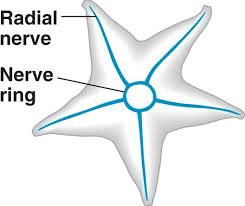
\includegraphics{figures/starfish.jpeg}
 \\
 \\
     \begin{subparts}
     \subpart[1]  Suppose you learn that the nerves in the arms only produce a response if their inputs exceeds a certain threshold. How would you represent this in your model?
     \fillwithlines{12em}
    \begin{soln}
    Any answer involving implementing ReLU activation functions, shifted or not, after each layer is correct.
    \end{soln}
    \begin{qauthor}
    Andrew, explain biological motivations of neural networks
    \end{qauthor}
     \subpart[1] Unfortunately, the left side of one of the arms is damaged, and can no longer produce a response from that side. How would you represent this in your model?
     \\
     \\
     \fillwithlines{12em}
    \begin{soln}
     For the affected arm, set the associated weights on one side of the associated neural network to be zero.
     \end{soln} 
     \begin{qauthor}
    Andrew, explain biological motivations of neural networks
    \end{qauthor}
     \\
     \\
     \subpart[2] You find that implementing five different neural networks is too much work, and decide to implement perceptrons in each arm instead. You may assume that as mentioned before, each one of their outputs is summed to produce the final response. Is this new representation of the response still characteristic of a non-linear neural network? If so, please explain in one concise sentence. If not, describe how you would change the setup described to mimic a neural network.
     \\
     \\
     \fillwithlines{12em}
     \begin{soln}
     It is not. Perceptrons and summation are both linear functions, so this setup does not characterize a non-linear neural network. To fix this, accept any answer that introduces non-linearity in the design.
     \end{soln} 
     \begin{qauthor}
    Andrew, Combine simpler models (e.g. linear regression, binary logistic regression, multinomial logistic regression) as components to build up feed-forward neural network architectures
    \end{qauthor}

     \end{subparts}



\end{parts}